\question{}

\begin{ابجد}
\item \textbf{نادرست}؛ تعداد گره‌های هرس شده، به مقدار اولین گرهی که در آن قسمت باز شده و همچنین به مقدار گره‌های قبلی بستگی دارد. مثال زیر را در نظر بگیرید:
\begin{figure}[H]
    \centering
    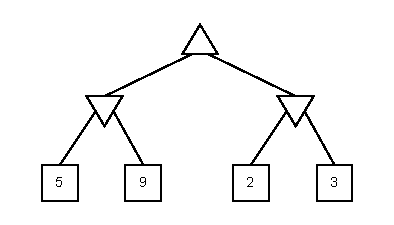
\includegraphics[width=0.5\textwidth]{assets/q1-A.pdf}
\end{figure}
اگر بخواهیم در هر مرحله گره‌ها را از چپ به راست بررسی کنیم، ابتدا بین مقادیر 5 و 9، 5 انتخاب می‌شود. سپس گره 2 باز شده و چون 2 از 5 کمتر است، گره 3 هرس می‌شود. اما اگر بخواهیم گره‌ها را از راست به چپ باز کنیم، بین 3 و 2، 2 انتخاب شده ولی بعد از باز شدن گره 9، $9 \nleq 2$ پس نمی‌توانیم گره آخر را هرس کنیم و باید باز شود.

\item \textbf{نادرست}؛ به عنوان نمونه ممکن است پس از کاهش دامنه‌ها با الگوریتم \lr{arc consistency} (مثل \lr{AC3})، یال‌های مسئله سازگار شوند (\lr{arc consistency}) ولی پاسخی وجود نداشته باشد. مثلاً در مسئله رنگ‌آمیزی نقشه، سه شهر دو‌به‌دو همسایه را در نظر بگیرید که هر یک فقط دو رنگ آبی و قرمز در دامنه خود دارند. در این حالت \lr{arc consistency} برقرار است، اما مسئله هیچ پاسخی ندارد. بنابراین همچنان به \lr{backtracking} نیاز داریم تا این موضوع را تشخیص دهیم.

اما با برقراری سازگاری تعمیم‌یافته (\lr{strong $n$-consistency}) می‌توان مسئله را بدون \lr{backtracking} حل کرد؛ هرچند در این حالت هم همچنان باید مقادیر متغیرها را به‌ترتیب انتخاب کنیم.

\item \textbf{نادرست}: مسائل \lr{CSP} به طور کلی در دسته مسائل \lr{NP-Complete} قرار می‌گیرند و در بدترین حالت برای حل کردن آنها نیاز به زمان نمایی داریم. تکنیک‌های \lr{MRV} و \lr{LCV} به همراه الگوریتم \lr{Arc Consistency} می‌توانند در بسیاری از موارد باعث شوند که به طور میانگین، تعداد \lr{backtrack} ها به شدت کاهش یابد. اما این روش‌ها در بدترین حالت نمی‌توانند مرتبه تعداد \lr{backtrack} ها را تغییر دهند. (اگر الگوریتم‌ها مشخص باشند، می‌توانیم مثالی بزنیم که تعداد \lr{backtrack} ها در آن از مرتبه $O(d^n)$ شود.)

\item \textbf{درست}: هنگامی که مسئله \lr{CSP} درختی باشد، یعنی بین گره‌های مختلف (که همان متغیرهای مسئله هستند) هیچ دوری وجود ندارد و بین دو گره مختلف حداکثر یک مسیر وجود دارد.

در این حالت، الگوریتم به این شکل است:
\begin{itemize}
    \item یک گره را به دلخواه به عنوان ریشه انتخاب کرده و گره‌ها را با ساختار درختی (از ریشه به برگ) مرتب می‌کنیم. ($O(n)$)
    \item از برگ‌ها شروع کرده و به سمت ریشه حرکت می‌کنیم. در هر مرحله، بررسی می‌کنیم که آیا به ازای هر مقدار در دامنه گره والد حداقل یک مقدار سازگار در دامنه هر فرزند آن وجود دارد یا خیر. اگر وجود نداشت، آن مقدار را از دامنه والد حذف می‌کنیم. ($O(nd^2)$)
    \item حال از ریشه شروع کرده، به سمت پایین حرکت می‌کنیم و برای هر گره، یکی از مقادیر سازگار با انتخاب‌های قبلی (والد) را انتخاب می‌کنیم. چون قبلاً سازگاری دامنه‌ها بررسی شده، در این مرحله نیازی به \lr{backtrack} نداریم و تمام گره‌ها مقداردهی می‌شوند. ($O(nd)$)
\end{itemize}

\item \textbf{نادرست}؛ می‌دانیم که در مسائل \lr{CSP} حالت‌های هدف زیرمجموعه‌ای از حالت‌های کامل هستند. الگوریتم \lr{BFS}، ابتدا تمام حالت‌های \lr{partial} را بررسی می‌کند تا در نهایت به حالت‌های کامل برسد؛ در حالی که الگوریتم \lr{DFS} حالت‌های کامل را زودتر بررسی می‌کند. بنابراین \lr{BFS} در مسائل \lr{CSP} عملکرد بدتری نسبت به \lr{DFS} دارد.

همچنین الگوریتم \lr{BFS} نیاز به فضای ذخیره‌سازی از مرتبه $O(d^n)$ دارد که مقدار بسیار زیادی است.

\item \textbf{نادرست}؛ ممکن است در یک مسئله ترتیب انتخاب متغیرها و اولویت مقادیری که به آنها می‌دهیم طوری باشد که الگوریتم \lr{backtracking} به سرعت یکی از پاسخ‌های درست را پیدا کند. در حالی که تلاش برای برقراری \lr{strong $k$-consistency} به مدت زمان زیادی نیاز داشته باشد.

\end{ابجد}